\documentclass[xcolor=table]{beamer}
\usepackage{fancyvrb}
\usepackage{fancybox}
\usepackage{listings}
\usepackage[utf8]{inputenc}
\usepackage{lmodern}
\graphicspath{ {imagenes/} }
\renewcommand{\tablename}{Tabla}
\renewcommand{\figurename}{Figura}
\usepackage{utopia}
\usepackage{graphics}
\usetheme{Madrid}
\usecolortheme{default}

\title[Estudio del cambio de representación en PA]
{Estudio del cambio de representación en planificación automática}

\subtitle{Trabajo fin de grado}

\author[Adrián Gil Moral] % (optional)
{Autor: Adrián Gil Moral \\ Tutora: Raquel Fuentetaja Pizán}

\institute[UC3M]
{
  Departamento de informática \\
  Universidad Carlos III de Madrid
}
\date[Julio 2017] % (optional)
{Julio 2017}

\titlegraphic{
\includegraphics[width=2cm,height=2cm]{uc3mLogo}}

%------------------------------------------------------------

%The next block of commands puts the table of contents at the 
%beginning of each section and highlights the current section:

\AtBeginSection[]
{
  \begin{frame}{Contenidos}
    \tableofcontents[currentsection]
  \end{frame}
}

\begin{document}

%---------------------------------------------------------

\frame{\titlepage}

%---------------------------------------------------------
\begin{frame}{Introducción}
    
    \begin{itemize}
        \item Área a la que pertenece el trabajo
        \begin{itemize}
            \item Inteligencia artificial
            \begin{itemize}
                \item Planificación automática
            \end{itemize}
        \end{itemize}
        \item Investigación
        
    \end{itemize}
\end{frame}

%---------------------------------------------------------

\begin{frame}{Problema Childsnack}

    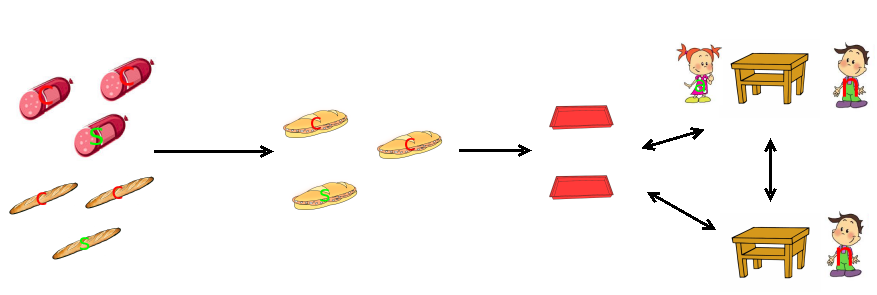
\includegraphics[width=12cm,height=8cm]{childSnack}
\end{frame}

%---------------------------------------------------------

\begin{frame}{Representación de Childsnack en planificación automática}
    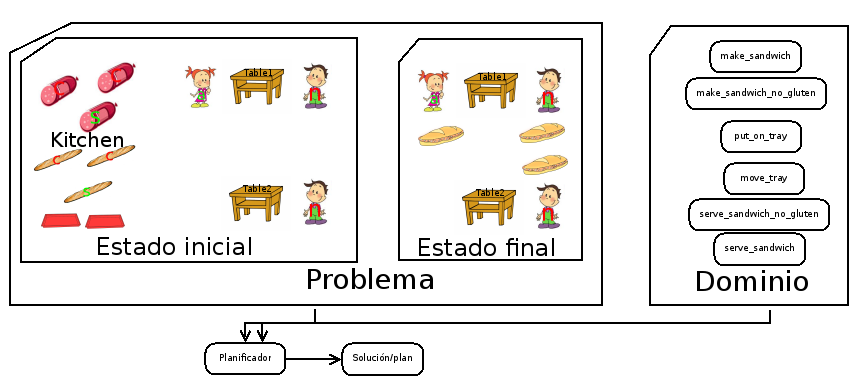
\includegraphics[width=12cm,height=8cm]{childSnack2}
\end{frame}

%---------------------------------------------------------

\begin{frame}{Representación en PDDL}
    \begin{columns}
        \column{0.3\textwidth}
        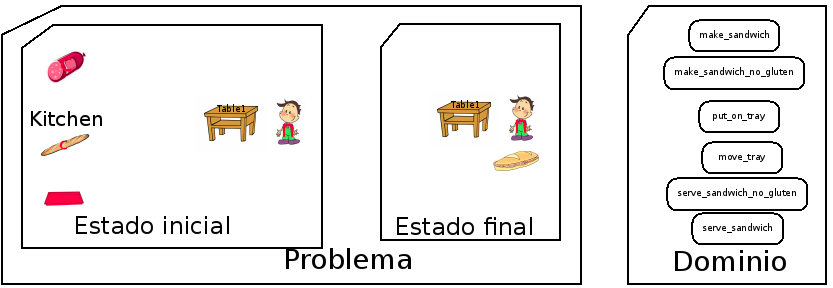
\includegraphics[width=4.5cm,height=3cm]{childSnack4}
        \begin{itemize}
            \item Estado inicial \\~\\
            \parbox{2in}{\shadowbox{
            \lstinputlisting[basicstyle=\tiny, linerange={1-5}]{codigo/cs.txt}
            }} \\~\\
            
            \item Estado final \\~\\
            \parbox{2in}{\shadowbox{
            \lstinputlisting[basicstyle=\tiny, linerange={6-6}]{codigo/cs.txt}
            }}
        \end{itemize}
        \column{0.5\textwidth}
        \begin{itemize}
            \item Operador del dominio \\~\\
            \parbox{2in}{\shadowbox{
            \lstinputlisting[basicstyle=\tiny, linerange={7-19}]{codigo/cs.txt}
            }} \\~\\
            \item Plan \\~\\
            \parbox{2in}{\shadowbox{
            \lstinputlisting[basicstyle=\tiny, linerange={20-23}]{codigo/cs.txt}
            }}
        \end{itemize}
    \end{columns}
\end{frame}

%---------------------------------------------------------

\begin{frame}{Cambios de representación en PDDL}
    \begin{itemize}
        \item Posibles modificaciones en los dominios y/o los problemas.
    \end{itemize}

    \begin{columns}
    \column{0.35\textwidth}
    \parbox{2in}{\shadowbox{
    \lstinputlisting[basicstyle=\tiny, linerange={7-19}]{codigo/cs.txt}
    }}
    
    \column{0.17\textwidth}
    \begin{flushright}
    
\includegraphics[width=1cm,height=1cm]{arrow}
    \end{flushright}
    
    \column{0.45\textwidth}
    \parbox{2in}{\shadowbox{
        \lstinputlisting[basicstyle=\tiny, linerange={1-21}]{codigo/cs2.txt}
        }}
    \end{columns}
    
\end{frame}

%---------------------------------------------------------

\begin{frame}{Motivación y objetivo}
    \begin{itemize}
        \item Motivación
        \begin{itemize}
            \item Investigación actualmente centrada en heurísticas
            \item Poco estudiado el impacto de la representación
            \item Actualmente es un problema abierto
        \end{itemize}
        \item Objetivo
        \begin{itemize}
            \item Medir el impacto de la variación en la representación de dominios en PDDL en el desempeño de distintos planificadores
        \end{itemize}
        \item Dominio utilizado para este fin: Childsnack
    \end{itemize}
    \begin{center}
        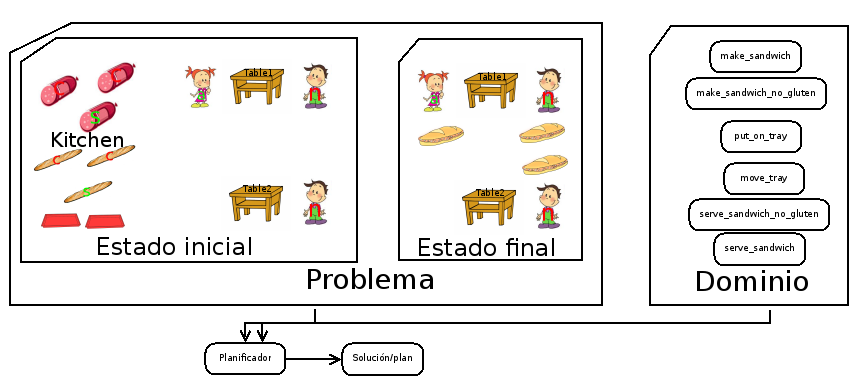
\includegraphics[width=5cm,height=3cm]{childSnack2}
    \end{center}
\end{frame}

%---------------------------------------------------------

\begin{frame}{Versiones de Childsnack utilizadas}
    \begin{itemize}
        \item \textbf{1} versión original del dominio de Childsnack de la IPC14
        \item \textbf{8} modificaciones realizadas a mano
        \item \textbf{3} modificaciones automáticas
    \end{itemize}
    \begin{center}
    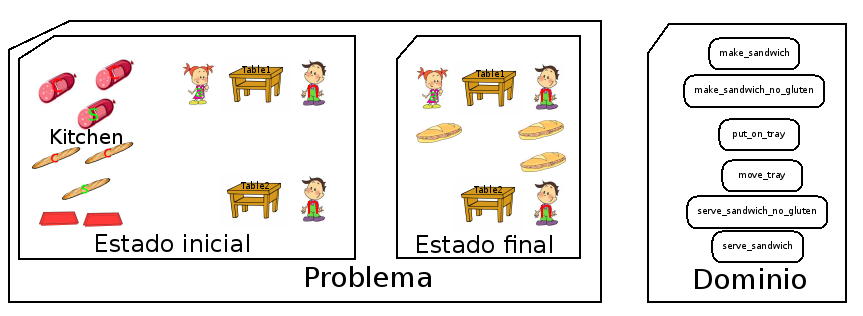
\includegraphics[width=6cm,height=4cm]{childSnack3}
    \end{center}
\end{frame}

%---------------------------------------------------------

\begin{frame}{Macrooperadores \{01, 03\}}
    \begin{itemize}
        \item Versión 01: unir los operadores move\_tray y serve\_sandwich\{-,\_no\_gluten\}
         \item Versión 03: el dominio contiene exclusivamente los operadores \texttt{make\_sandwich\_move\_tray\_serve\_sandwich\_no\_gluten\_move\_tray} \texttt{\_kitchen}, \texttt{make\_sandwich\_move\_tray\_serve\_sandwich\_move\_tray\_kitchen} y \texttt{move\_tray\_kitchen}
    \end{itemize}
\end{frame}

%---------------------------------------------------------

\begin{frame}{Precondiciones en los operadores \{02\}}
    
    \begin{itemize}
    
        \item Modificación del operador \texttt{make\_sandwich} para que no acepte la entrada de pan y contenido sin gluten
    \end{itemize}
    
    \parbox{2in}{\shadowbox{
        \lstinputlisting[basicstyle=\tiny]{codigo/v02.txt}
        }}

\end{frame}

%---------------------------------------------------------

\begin{frame}{Versiones numéricas \{05, 08, numDigits\}}
    \begin{itemize}
        \item Pasar a formato numérico los predicados \texttt{at\_kitchen\_}\{bread, content, sandwich\} y definirlos bien con proposiciones, bien con funciones numéricas
        \item En el caso de la versión manual con proposiciones, añadir predicados \texttt{next} (\texttt{(next num0 num1)} \texttt{(next num1 num2)})
    \end{itemize}
    \parbox{2in}{\shadowbox{
        \lstinputlisting[basicstyle=\tiny]{codigo/vNum.txt
        }}}
\end{frame}

%---------------------------------------------------------

\begin{frame}{Versión numProps}
    \begin{itemize}
        \item La representación de este dominio varía por completo respecto a la versión manual (v08)
        \item Generada por Baggy
    \end{itemize}
\end{frame}

%---------------------------------------------------------

\begin{frame}{Macropredicados \{09\}}
    \begin{columns}
    
    \column{0.25\textwidth}
    \parbox{2in}{\shadowbox{
    \lstinputlisting[basicstyle=\tiny, linerange={1-1}]{codigo/v09.txt}
    }}
    \parbox{2in}{\shadowbox{
    \lstinputlisting[basicstyle=\tiny, linerange={2-2}]{codigo/v09.txt}
    }}
    \parbox{2in}{\shadowbox{
    \lstinputlisting[basicstyle=\tiny, linerange={4-4}]{codigo/v09.txt}
    }}
    \parbox{2in}{\shadowbox{
    \lstinputlisting[basicstyle=\tiny, linerange={5-5}]{codigo/v09.txt}
    }}
    
    \column{0.17\textwidth}
    \begin{flushright}
    
\includegraphics[width=1.5cm,height=1.5cm]{arrow}
    \end{flushright}
    
    \column{0.43\textwidth}
    \parbox{2in}{\shadowbox{
    \lstinputlisting[basicstyle=\tiny, linerange={3-3}]{codigo/v09.txt}
    }}
    \parbox{2in}{\shadowbox{
    \lstinputlisting[basicstyle=\tiny, linerange={6-6}]{codigo/v09.txt}
    }}
    \end{columns}
\end{frame}

%---------------------------------------------------------

\begin{frame}{Hipótesis del mundo cerrado \{v11\}}
    \begin{itemize}
        \item Hipótesis del mundo cerrado: todo hecho no definido es negativo
        \item Cambiar predicados \texttt{(not\_allergic\_gluten)} y \texttt{(served)} por \texttt{not(allergic\_gluten)} y \texttt{not(waiting)} respectivamente
        
    \end{itemize}
    
\end{frame}

%---------------------------------------------------------

\begin{frame}{Ejecución por etapas \{v12\}}
    \begin{itemize}
        \item Etapas:
        \begin{enumerate}
            \item \texttt{a} = #niños alérgicos que hay que servir
            \item \texttt{b} = #niños no alérgicos que hay que servir
            \item Hacer \texttt{a} sándwiches sin gluten
            \item Hacer \texttt{b} sándwiches con gluten
            \item Si no existe ninguna bandeja en la cocina, mover bandeja \texttt{c} a la cocina
            \item Cargar \texttt{a, b} sándwiches en \texttt{c}
            \item Para cada localización \texttt{d} en la que haya un niño que tenga que ser servido:
            \begin{itemize}
                \item Mover \texttt{c} a \texttt{d}
                \item Para cada niño en \texttt{d} que falte por servir, servir sándwich \texttt{a}/\texttt{b} a \texttt{d} según sus necesidades alérgicas
            \end{itemize}
        \end{enumerate}
    \end{itemize}
\end{frame}

%---------------------------------------------------------

\begin{frame}{Optimalidad y completitud}
    \begin{table}[]
\centering
\label{my-label}
\begin{tabular}{|c|c|c|}
\hline
\textbf{}          & \textbf{Completa} & \textbf{Óptima} \\ \hline
\textbf{V01}       & Sí                & Sí              \\ \hline
\textbf{V02}       & Sí                & Sí              \\ \hline
\textbf{V03}       & \textbf{No}                & \textbf{No}              \\ \hline
\textbf{V05}       & Sí                & Sí              \\ \hline
\textbf{V08}       & Sí                & Sí              \\ \hline
\textbf{V09}       & Sí                & Sí              \\ \hline
\textbf{V11}       & Sí                & Sí              \\ \hline
\textbf{V12}       & \textbf{No}                & Sí              \\ \hline
\textbf{numProp}   & Sí                & Sí              \\ \hline
\textbf{numDigits} & Sí                & Sí              \\ \hline
\end{tabular}
\end{table}
\end{frame}

%---------------------------------------------------------

\begin{frame}{Entorno experimental}
    \begin{itemize}
        \item Ejecución
        \begin{itemize}
            \item Planificadores MFF, LPG-td y FD
            \item 30 minutos/problema como límite
            \item 20 problemas de Childsnack de la IPC14 redefinidos según cada representación
        \end{itemize}
        \item Métricas
        \begin{itemize}
            \item Número de problemas resueltos
            \item Tiempo de ejecución
            \item Calidad de la solución
        \end{itemize}
    \end{itemize}
\end{frame}

%---------------------------------------------------------
\begin{frame}{Resultados MFF coste v12}
    \begin{center}
    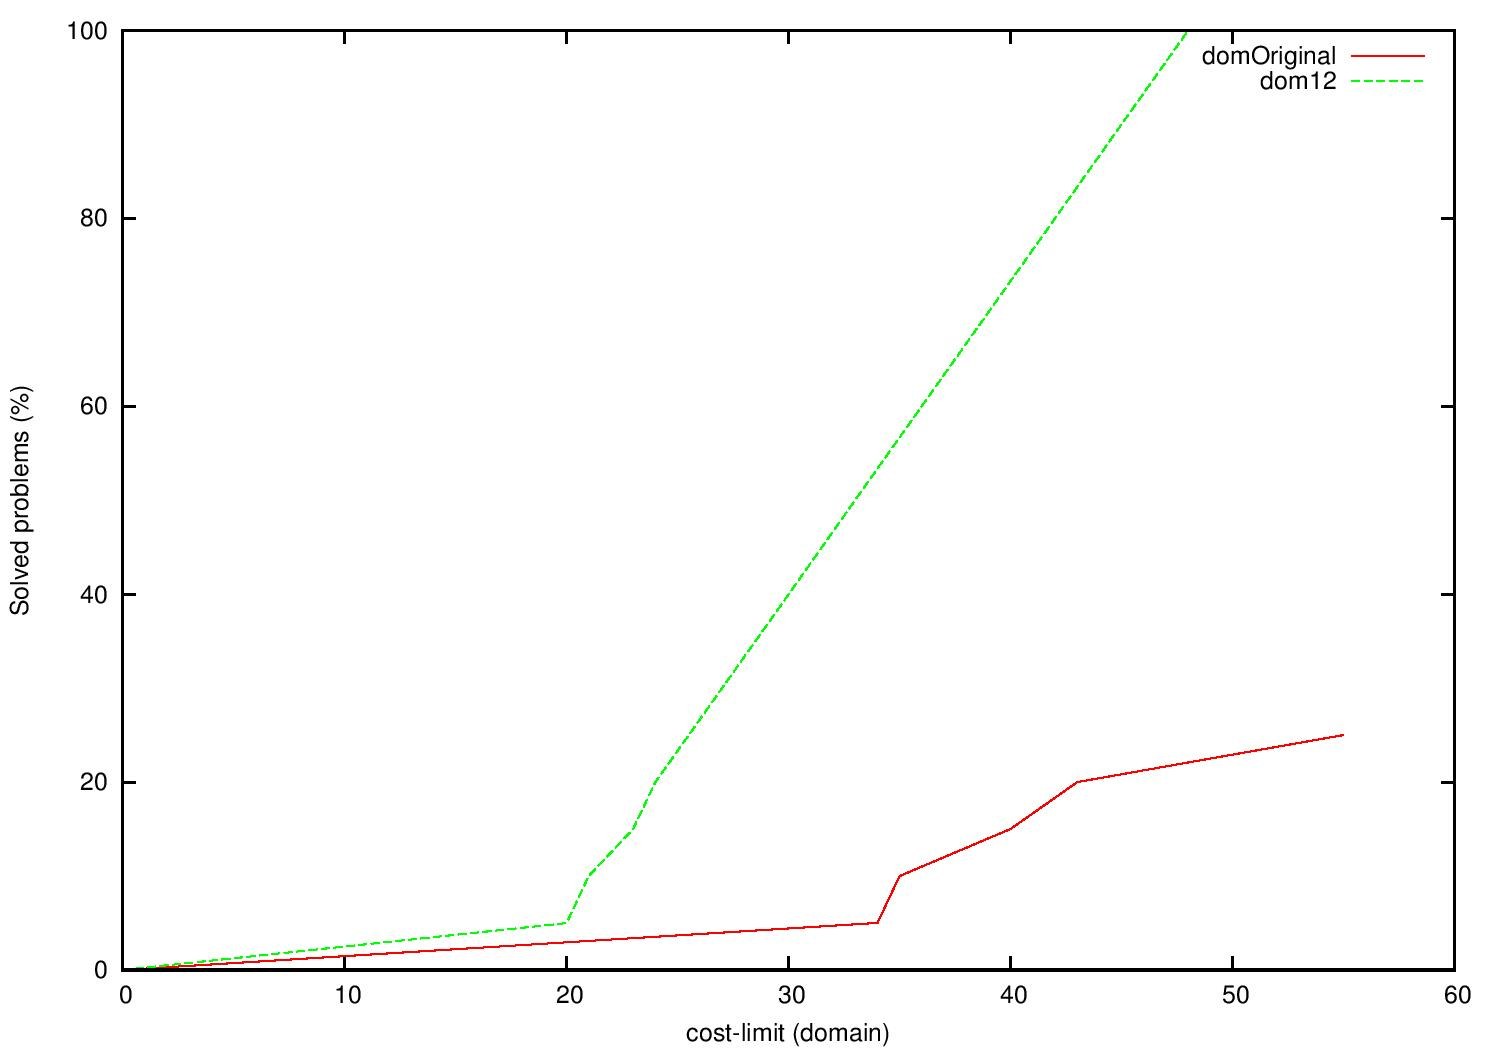
\includegraphics[width=7cm, height=7cm]{mff-or-12-cost}
    \end{center}
\end{frame}

%---------------------------------------------------------

\begin{frame}{Resultados LPG-td coste v12}
    \begin{center}
    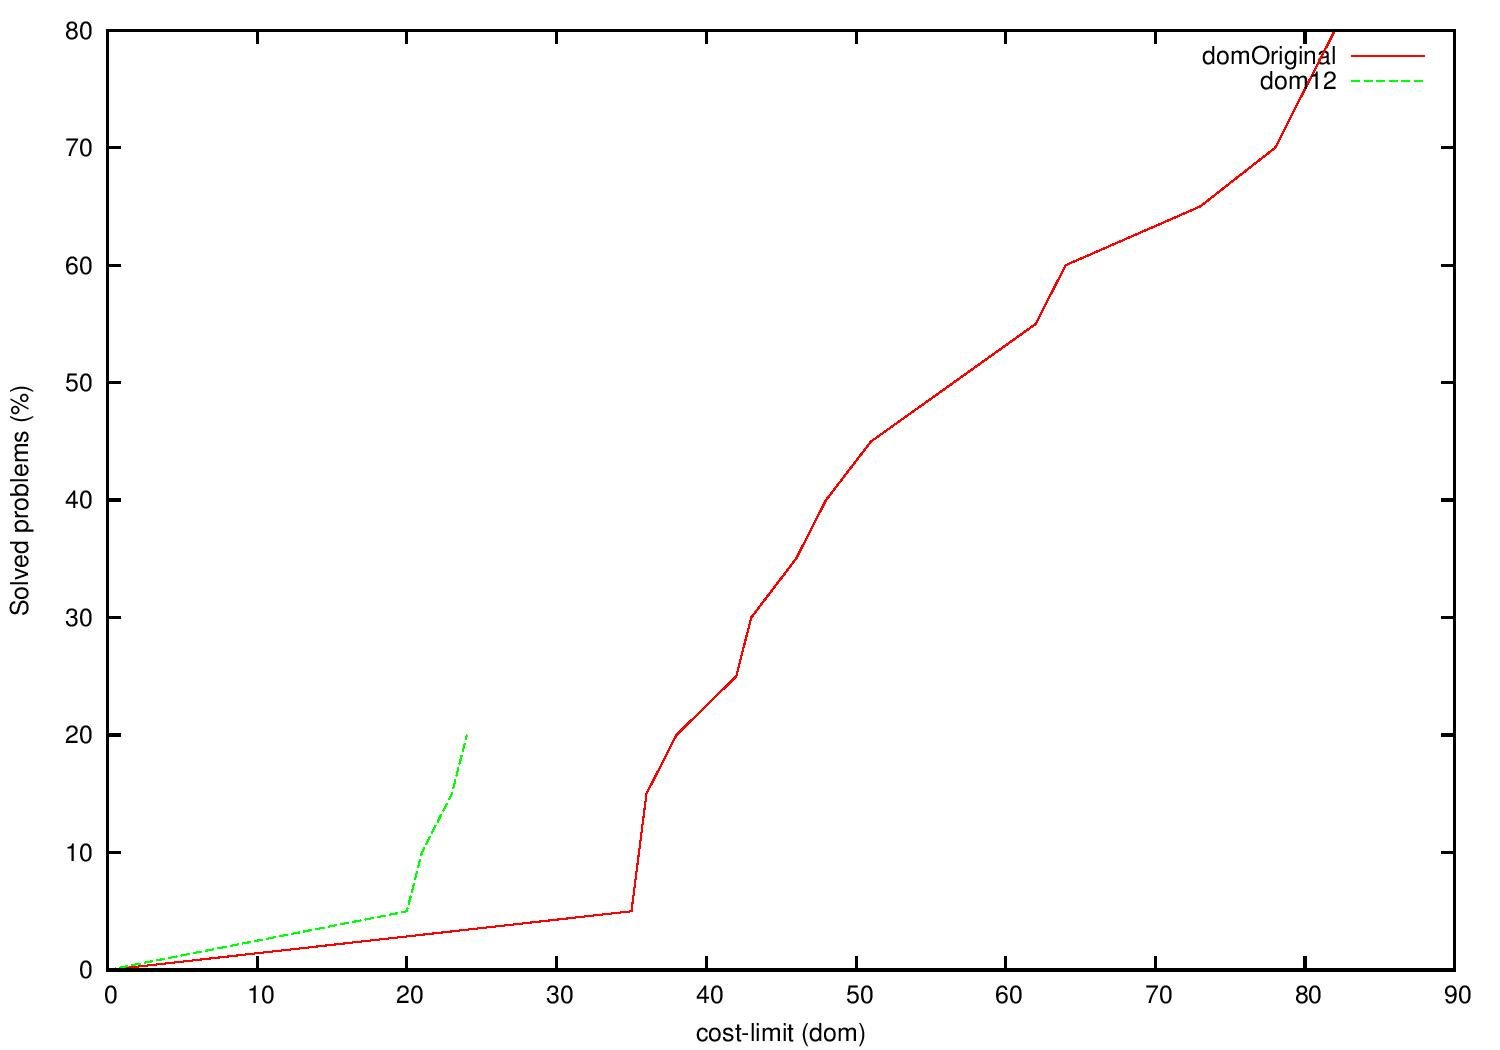
\includegraphics[width=7cm, height=7cm]{lpg-or-12-cost}
    \end{center}
\end{frame}

%---------------------------------------------------------

\begin{frame}{Resultados globales}
    \begin{table}[]
\centering
\scalebox{0.65}{
\begin{tabular}{|c|c|c|c|c|c|c|}
\hline
\textbf{Versiones}                 & \textbf{Tiempo MFF} & \textbf{Calidad MFF} & \textbf{Tiempo LPG-td} & \textbf{Calidad LPG-td} & \textbf{P.MFF} & \textbf{P.LPG-td} \\ \hline
\textbf{original}  & 0,126                   & 0,200                    & 0,611                     & 0,689                       & 6º                      & 6º                         \\ \hline
\textbf{v01}       & 0,981                   & 0,871                    & 0,584                     & 0,708                       & \cellcolor{blue!25}1º                      & \cellcolor{blue!25}7º                         \\ \hline
\textbf{v02}       & 0,121                   & 0,200                    & 0,690                     & 0,863                       & 9º                      & 5º                         \\ \hline
\textbf{v03}       & 0,074                   & 0,148                    & 0,802                     & 0,982                       & 10º                     & 4º                         \\ \hline
\textbf{v05}       & 0,572                   & 0,778                    & 0,052                     & 0,189                       & 4º                      & 10º                        \\ \hline
\textbf{v08}       & 0,024                   & 0,085                    & 1,000                     & 0,839                       & 11º                     & 3º                         \\ \hline
\textbf{v09}       & 0,124                   & 0,200                    & 0,935                     & 0,967                       & \cellcolor{blue!25}7º                      & \cellcolor{blue!25}1º                         \\ \hline
\textbf{v11}       & 0,121                   & 0,202                    & 0,917                     & 0,958                       & 7º                      & 2º                         \\ \hline
\textbf{v12}       & 0,723                   & 0,999                    & 0,109                     & 0,200                       & \cellcolor{blue!25}2º                      & \cellcolor{blue!25}9º                         \\ \hline
\textbf{numProps}  & 0,567                   & 0,948                    & 0,023                     & 0,050                       & 3º                      & 11º                        \\ \hline
\textbf{numDigits} & 0,137                   & 0,218                    & 0,304                     & 0,837                       & 5º                      & 8º                         \\ \hline
\end{tabular}}
\end{table}

\begin{itemize}
    \item El índice de correlación de Pearson para los tiempos obtenidos con MFF y LPG-td es de \textbf{-0,6256}
\end{itemize}

\end{frame}

%---------------------------------------------------------

\begin{frame}{Conclusiones}
    \begin{itemize}
        \item Existe correlación entre representación y el desempeño de la planificación
        \item El planificador usado influye en la idoneidad de una representación
        \item Amplio margen de mejora en los modificadores automáticos de representación
    \end{itemize}
\end{frame}

%---------------------------------------------------------

\begin{frame}{Trabajo futuro}
    \begin{itemize}
        \item Ampliación de las pruebas con más planificadores y tipos de problemas
        \item Estudio de los tipos representaciones más adecuadas para cada tipo de planificador
        \item A largo plazo:
        \begin{itemize}
            \item Modificador automático en función del planificador
            \item Planificador de tipo portfolio que elija el planificador más adecuado según la representación
        \end{itemize}
        
    \begin{center}
        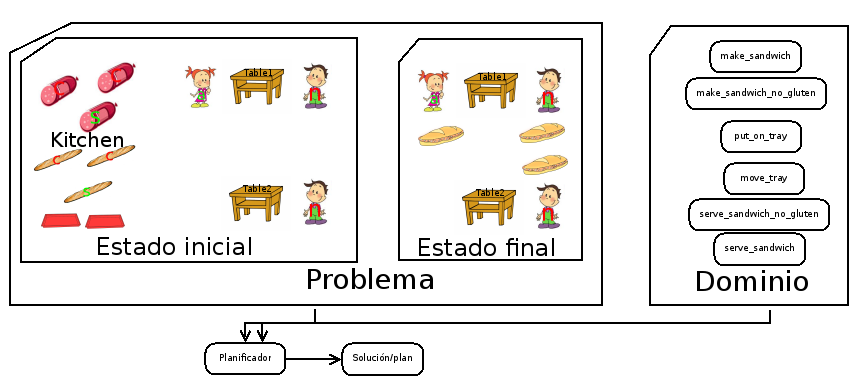
\includegraphics[width=5cm,height=3cm]{childSnack2}
    \end{center}
        
    \end{itemize}
\end{frame}


%---------------------------------------------------------

\end{document}